\documentclass[12pt, a4paper]{article}
\usepackage{polski}
\usepackage{indentfirst}
\usepackage{listings}
\usepackage{graphicx}
\usepackage{geometry}
\usepackage{hyperref}
\usepackage{csquotes}
\hypersetup{
    colorlinks=true,
    linkcolor=black,
    filecolor=magenta,      
    urlcolor=cyan,
}
 
\urlstyle{same}

\lstset{
 columns=fullflexible,
  frame=single,
  breaklines=true,
  postbreak=\mbox{{$\hookrightarrow$}\space},
  literate=%
{ą}{{\k{a}}}1
{Ą}{{\k{A}}}1
{ć}{{\'c}}1
{Ć}{{\'{C}}}1
{ę}{{\k{e}}}1
{Ę}{{\k{E}}}1
{ł}{{\l{}}}1
{Ł}{{\L{}}}1
{ń}{{\'n}}1
{Ń}{{\'N}}1
{ó}{{\'o}}1
{Ó}{{\'O}}1
{ś}{{\'s}}1
{Ś}{{\'S}}1
{ż}{{\.z}}1
{Ż}{{\.Z}}1
{ź}{{\'z}}1
{Ź}{{\'Z}}1
}
\usepackage[utf8]{inputenc}
%nagłówek i stopka:
\usepackage{lastpage}
\usepackage{fancyhdr}
\pagestyle{fancy}
\fancyhf{}
\lhead{Business Intelligence (BI) – sztuczna inteligencja w systemach biznesowych}
\cfoot{\thepage \ z \pageref{LastPage}}

%nagłówek na stronie tytułowej -> musi być specjalny, żeby przesłonić :)
\fancypagestyle{firstPageStyle}{
\fancyhf{}
\cfoot{\thepage \ z \pageref{LastPage}}
\renewcommand{\footrulewidth}{0.5pt} % Line at the footer visible
}

\title{Sprawozdanie na przedmiot Kompresja Danych, implementacja algorytmu LZW.}
\author{Bartosz Puszkarski}
\date{Grudzień 2019}

\begin{document}

\maketitle
\thispagestyle{firstPageStyle}
\newpage
\tableofcontents

\newpage

\section{Wstęp}
Celem projektu było zaimplementowanie dowolnego algorytmu kompresji bestratnej, które docelowym obszarem działań będą pliki tekstowe. Pozwolono nam na wybór języka i środowiska implementacji wybranej metody, wybór ograniczono do dwóch opcji - Matlab lub Python.\\
Po zapoznaniu się z materiałem przedstawionym na wykładzie oraz uzupełniając informacje w oparciu o źródła internetowe zdecydowałem się na implementację algorytmu bezstratnej kompresji słownikowej w wersji uproszczonej \textbf{LZW}.

\section{Omówienie teoretyczne algorytmu LZW}
Metoda LZW jest modyfikacją swojej poprzedniczki, metody LZ78. Dziedziczy po niej zasady działania. W metodzie tej, słownik inicjalizowany jest alfabetem kodowanego ciągu, a elementarne składniki zbioru (\textit{elementy podstawowe}) są znane i uporządkowane w taki sposób, że każdy element podstawowy ma ustalony poprzednik i następnik. \\
Głównym powodem, dla którego wybrałem właśnie tę metodę jest fakt, że udało mi się ją przyswoić najszybciej i wydawała mi się najbardziej intuicyjna. 
\subsection{Cechy metody LZW}
\begin{itemize}
\item Daje lepsze wyniki niż LZ78 (słownik szybko się zapełnia),
\item Dane wyjściowe składają się jedynie z indeksów w słowniku,
\item Możliwość wystąpienia przypadku szczególnego: kodowanie pozycji w słowniku, która nie została jeszcze zapełniona - wymaga odpowiedniej modyfikacji algorytmu.
\item Najlepiej koduje krótkie sekwencje danych,
\end{itemize}
\subsection{Algorytm LZW}
Aby w najprostszy i najczytelniejszy sposób przedstawić działanie algorytmu posłużę się listą kroków dostarczoną nam podczas wykładu przez prof. Raka.
\begin{itemize}
\item Wypełnienie słownika alfabetem kodowanej informacji,
\item Wczytanie znaku z wejścia,
\item Jeśli znak połączony z ostatnio wczytanymi (o ile były) da frazę, która znajduje się w słowniku, wyemituj jej indeks, a do pamięci zapisz ostatni znak z wejścia, który nie pasował do frazy ze słownika.
\item Dopisanie do słownika frazy powstałej z połączenia znaku w pamięci i wczytanych znaków.
\item Powtarzanie tego procesu aż do wyczerpania strumienia wejściowego.
\end{itemize}
\section{Projekt i działanie programu}
\subsection{Projekt}
Program został skonstruowany w sposób modularny, gdzie moduł główny, w procesie realizacji celów projektowych, posługuje się klasą \textbf{LZW}, w której został zaimplementowany algorytm kompresji i dekompresji z wykorzystaniem metody LZW.

\begin{figure}[!ht]
    \centering
    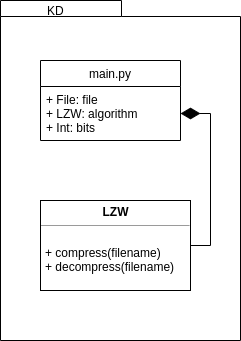
\includegraphics[scale=0.75]{uml.png}
    \caption{Podział modułowy programu.}
    \label{fig:MODULES}
\end{figure}

Program ograniczony został jedynie do działania w trybie wsadowym.
Aby zapewnić prostotę obsługi została także zaimplementowana pomoc.
\begin{verbatim}
->  kompresja-projekt python3 main.py -h
usage: main.py [-h] [-c] [-d] FILE BITS

Implementacja algorytmu kompresji słownikowej bezstratnej LZW, wykonana w
języku Python v3.6, jako projekt na Podstwy Kompresji Danych laboratoria.
Należy skorzystać tylko i wyłącznie z jednego trybu pracy programu na raz.

positional arguments:
  FILE        nazwa pliku, który chcemy skompresować / zdekompresować
  BITS        ilość bitów wykorzystywana do określenia maksymalnej pojemności
              słownika (nie zaleca się korzystania z liczb poniżej 8)

optional arguments:
  -h, --help  show this help message and exit
  -c          Tryb pracy - kompresja
  -d          Tryb pracy - dekompresja

\end{verbatim}
\subsection{Implementacja}
\subsubsection{Moduł główny - main.py}
W module głównym \textbf{main.py} następuje użytych flag:
\begin{verbatim}
if args.decompress and args.compress:
    raise ValueError("Wybrano więcej niż jeden tryb pracy")
\end{verbatim}

oraz wywołanie pożądanej funkcjonalności:
\begin{verbatim}
if args.compress:
    algorithm.compress(args.filename)
elif args.decompress:
    algorithm.decompress(args.filename)
\end{verbatim}

\subsubsection{Algorytm LZW}
Algorytm został zaimplementowany w klasie \textbf{LZW} w obu trybach pracy - kompresji oraz dekompresji.\\
Implementacja głównej części algorytmu realizującej \textbf{kompresję}:
\begin{verbatim}
for symbol in data:
    recent_chain_with_next_symbol = recent_chain + symbol
    if recent_chain_with_next_symbol in self.dictionary:
        recent_chain = recent_chain_with_next_symbol
    else:
        compressed_data.append(self.dictionary[recent_chain])
        if(len(self.dictionary) <= self.max_table_size):
            self.dictionary[recent_chain_with_next_symbol] = self.dict_size
            self.dict_size += 1
        recent_chain = symbol
if recent_chain in self.dictionary:
    compressed_data.append(self.dictionary[recent_chain])
\end{verbatim}
Oczywiście kompresja ta realizowana jest po uprzednim zainicjowaniu słownika zgodnie z zasadami metody:
\begin{verbatim}
self.dictionary = {chr(i): i for i in range(dict_size)}
\end{verbatim}

Następnie skompresowane dane są zapisywane do pliku, o nazwie tożsamej nazwie pliku danych wejściowych z rozszerzeniem \textbf{*.lzw}, w postaci bitów zapisanych z kodowaniem hexadecymalnym:
\begin{verbatim}
self.compressed_data = compressed_data
output_file = open(filename.split('.')[0] + '.lzw', "wb")
for data in self.compressed_data:
    output_file.write(pack('>H', int(data)))
output_file.close()
\end{verbatim}

\vspace{1cm}
Implementacja algorytmu \textbf{LZW} realizująca dekompresję podanego pliku w formacie \textbf{*.lzw}. (Program był testowany jedynie na pliku stworzonym przez przez swoją instancję - rezultat wywołania metody \textit{compress()} ).
\begin{verbatim}
for code in compressed_data:
    if not (code in dec_dictionary):
        dec_dictionary[code] = recent_chain + recent_chain[0]
    decompressed_data += dec_dictionary[code]
    if not(len(recent_chain)) == 0:
        dec_dictionary[next_code] =recent_chain + (dec_dictionary[code][0])
        next_code += 1
    recent_chain = dec_dictionary[code]
\end{verbatim}
Tak jak w przypadku kompresji, tutaj także wyżej przedstawiona część realizowana jest w oparciu o wcześniej inicjowany słownik:
\begin{verbatim}
dec_dictionary = {i: chr(i)) for i in range(dec_dict_size)}
\end{verbatim}

Ponieważ dekompresowane dane pochodzą z pliku, którego treść została zakodowana w systemie hexadecymalnym istnieje konieczność odkodowania danych wejściowych. Podstawą operacji jest odczytywanie par znaków z pliku wejściowego, dekodowanie ich i dodawanie do tablicy.
\begin{verbatim}
while True:
    rec = f.read(2)
    if len(rec) != 2:
        break
    (data, ) = unpack('>H', rec)
    compressed_data.append(data)
\end{verbatim}

Otrzymane zdekompresowane dane zapisywane są w pliku o nazwie tożsamej z plikiem wejściowym z dodanym sufiksem \textbf{decompressed} w formacie \textbf{*.txt}:
\begin{verbatim}
out = filename.split('.')[0] + "_decompressed.txt"
output_file = open(out, 'w')
for data in decompressed_data:
    output_file.write(data)
output_file.close()

\end{verbatim}

\section{Podsumowanie i obserwacje}
W trakcie testowania programu zauważyłem ciekawe zachowanie w przypadku podania za małej liczby bitów złóżących do określania wielkości - gdy podano liczbę mniejszą od 8, wielkość słownika była mniejsza niż 256 pozycji a plik wynikowy był 2x większych rozmiarów, niż plik źródłowy, który miał zostać skompresowany. Oczywiście wynik kompresji był nie do odkodowania, więc zakładam, że zwyczajnie był zły.
Udało mi się osiągnąć kompresję często-powtarzającego się tekstu zawartego w pliku testowym na poziomie 50\%.

\end{document}


